\documentclass{article}
\usepackage{amsmath}
\usepackage{amssymb}
\usepackage{graphicx}
\usepackage{hyperref}
\usepackage[version=4]{mhchem}


\begin{document}
\(A B C D\) is a convex quadrilateral. \(A B=C D . E, F\) are midpoints of \(B C, A D\), respectively. The extensions of \(B A\) and \(C D\) meet the extension of \(E F\) at \(M, N\), respectively. Show that \(\angle B M E\) \(=\angle C N E\).

Solution:
Method 1:\\
Connect \(B D\). Take \(G\), the midpoint of \(B D\). Connect \(G F, G E\).\\
\centering
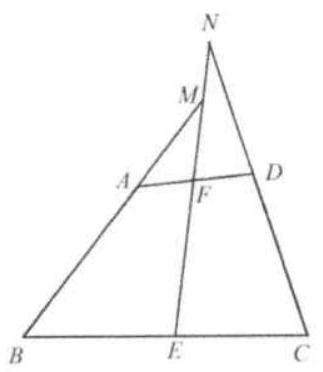
\includegraphics[width=\textwidth]{images/042(2).jpg}

Since \(G F\) is the midline of \(\triangle D A B\).\\
\(G F / / A B\) and \(G F=\frac{1}{2} A B\)\\
\(G E\) is the midline of \(\triangle B D C\).\\
\(G E / / C D\) and \(G E=\frac{1}{2} C D\).\\
Since \(A B=C D, G F=G E\).\\
\centering
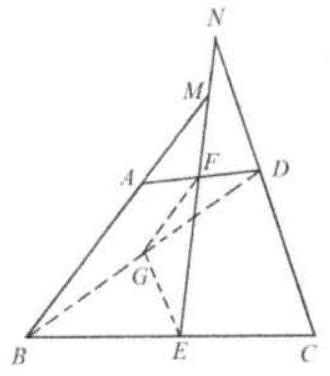
\includegraphics[width=\textwidth]{images/042.jpg}

Thus \(\angle G F E=\angle G E F\).\\
We know that \(G F / / A B\), so \(\angle B M E=\angle G F E\).\\
We also know that \(G E / / C D / / C N\), so \(\angle C N E=\angle G E F\)\\
Therefore, \(\angle B M E=\angle C N E\).

Method 2:\\
Connect \(A C\). Take \(P\), the midpoint of \(A C\). Connect \(E P, E P\).\\
Since \(E P\) is the midline of \(\triangle C A B, E P / / A B\) and \(E P=\frac{1}{2} A B\).\\
\(F P\) is the midline of \(\triangle A D C\).\\
\(F P / / C D\) and \(F P=\frac{1}{2} C D\).\\
\centering
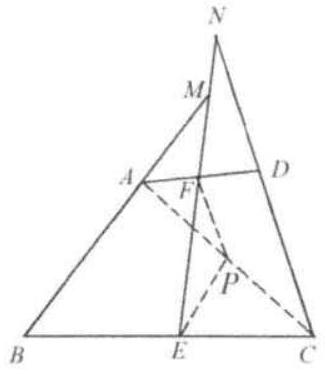
\includegraphics[width=\textwidth]{images/043.jpg}

Since \(A B=C D, E P=F P\). Thus \(\angle P F E=\angle P E F\).\\
We know that \(E P / / A B\), so \(\angle B M E=\angle P E F\).\\
We also know that \(F P / / C D / / C N\), so \(\angle C N E=\angle P F E\)\\
Therefore, \(\angle B M E=\angle C N E\).
\end{document}
